\begin{figure}
  \setlength{\unitlength}{\textwidth}

        \begin{picture}(1,1)(0,0.35)

      % % % Parkinson Data 
      \put(0,1.5){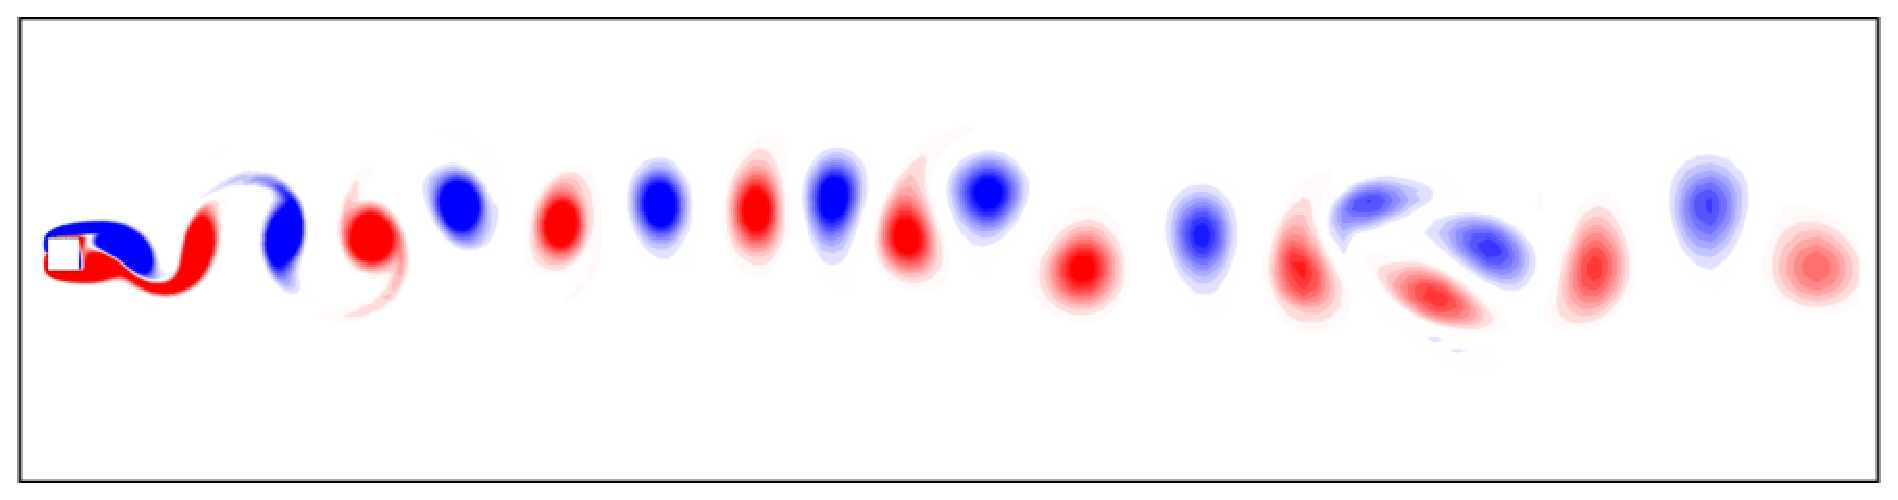
\includegraphics[width=1\unitlength]{../FnP/gnuplot/10.eps}}
      \put(0,1.16){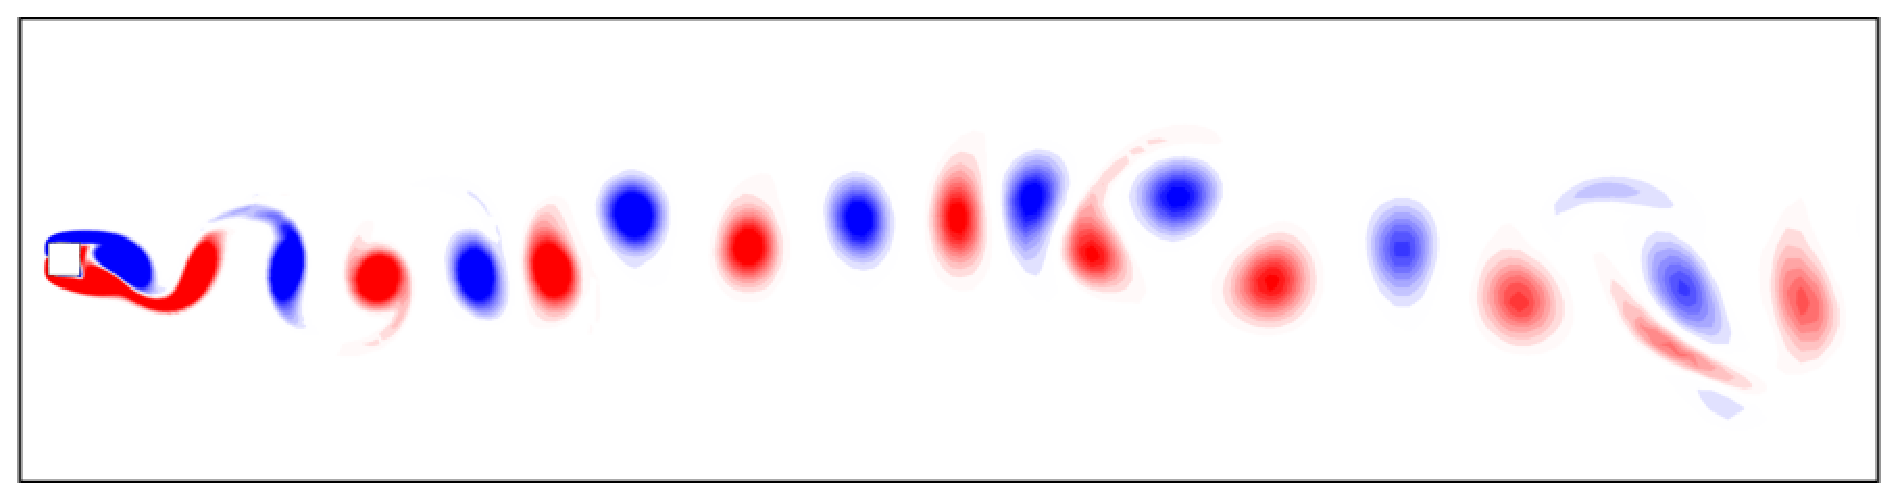
\includegraphics[width=1\unitlength]{../FnP/gnuplot/60.eps}}
      \put(0,0.82){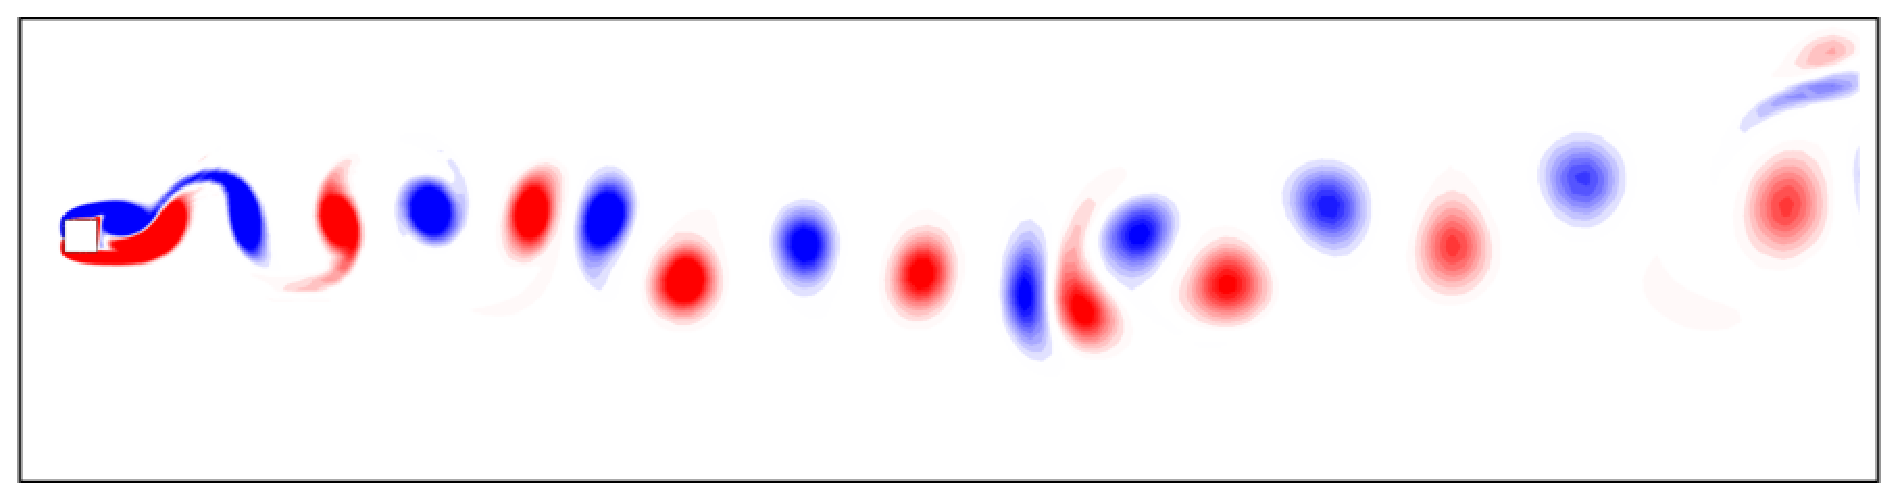
\includegraphics[width=1\unitlength]{../FnP/gnuplot/250.eps}}
      \put(0,0.47){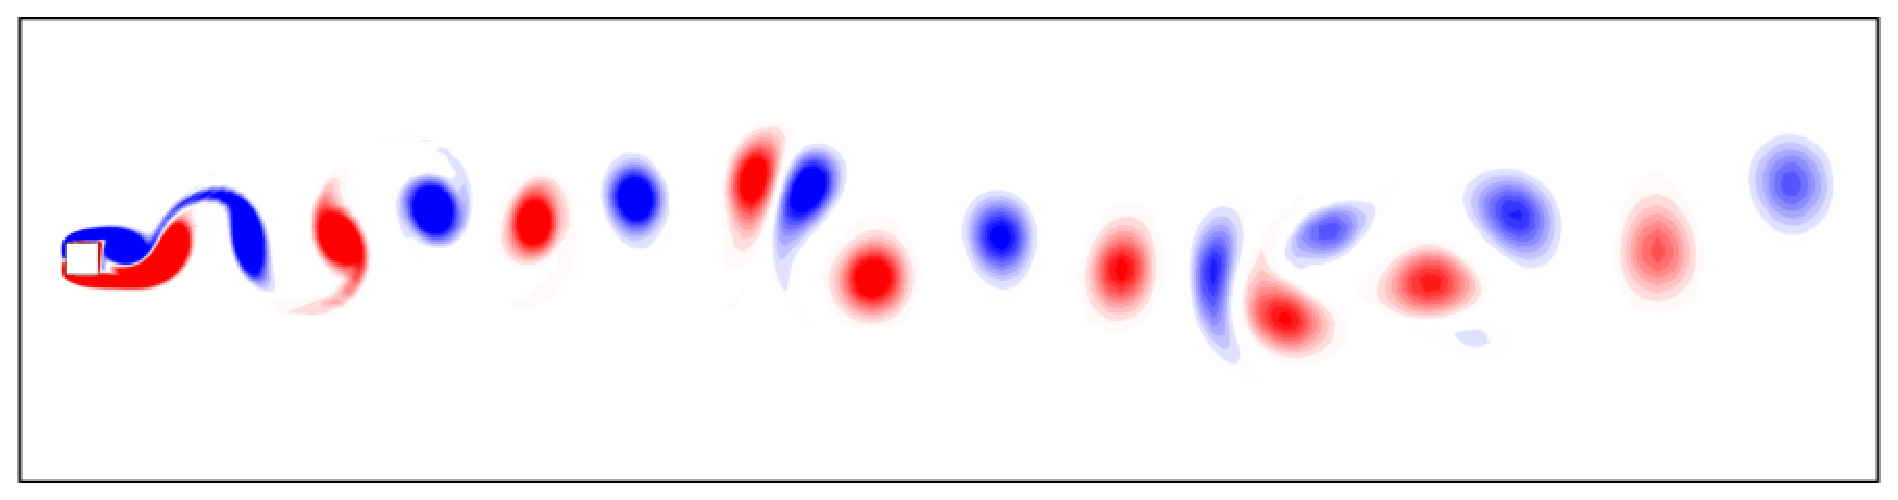
\includegraphics[width=1\unitlength]{../FnP/gnuplot/1000.eps}}
      
      



%      
    \put(0.01,1.72){\small(a)}
     \put(0.01,1.38){\small(b)}
     \put(0.01,1.04){\small(c)}
 	\put(0.01,0.69){\small(d)}
      
    \end{picture}

    \caption{Vorticity plots of the flow at arbitrary positions at $\massdamp=0.47$. (a) $\massstiff=10$, (b) $\massstiff=60$ 
    	(c) $\massstiff=250$ and (d) $\massstiff=1000$ at $\reynoldsnumber=200$.}
    \label{fig:qss_fsi}
\end{figure}

 %vspace{10cm}
